\documentclass[11pt, oneside]{article} 
\usepackage{geometry}
\geometry{letterpaper} 
\usepackage{graphicx}
	
\usepackage{amssymb}
\usepackage{amsmath}
\usepackage{parskip}
\usepackage{color}
\usepackage{hyperref}

\graphicspath{{/Users/telliott_admin/Dropbox/Tex/png/}}
% \begin{center} 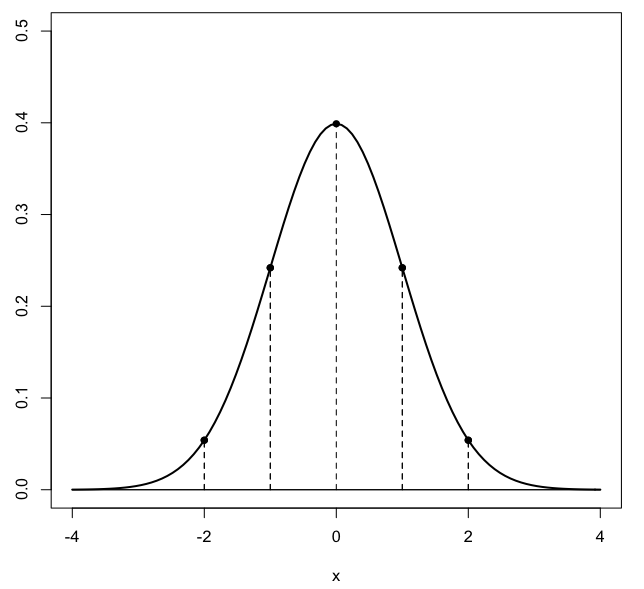
\includegraphics [scale=0.4] {gauss3.png} \end{center}

\title{Square root of 3}
\date{}

\begin{document}
\maketitle
\Large
Archimedes uses two approximations for $\sqrt{3}$:  $265/153$  and $1350/780$. (Recall that $\sqrt{3}$ is irrational so it doesn't have an exact decimal representation). 

I wrote a script to search for these and other close approximations.

\begin{verbatim}
> python approx_sqrt3.py 
     0      0      0      1      1
     1      1      2      2      1
     3      5      2      6      9
     4      6     12      7      1
    11     19      2     20     37
    15     25     50     26      1
    41     71      2     72    141
    56     96    192     97      1
   153    265      2    266    529
   209    361    722    362      1
   571    989      2    990   1977
   780   1350   2700   1351      1
  2131   3691      2   3692   7381
  2911   5041  10082   5042      1
  7953  13775      2  13776  27549
 10864  18816  37632  18817      1
> 
\end{verbatim}
The first column has the denominator $i$ (we search from 1 to 50000).  

The algorithm is really brute force.  For each possible $i$, we search all the integers larger than $i$ until we find one $j$ such that $3 \cdot i^2 < j^2$.  In other words, $j$ is the smallest integer such that $j/i$ is larger than $\sqrt{3}$.  

Having the closest $j$ (and $j-1$) for each $i$, we test whether
\[ j^2 - 3 \cdot i^2 < 5 \]
\[ 3 \cdot i^2 - (j-1)^2 < 5 \]

If eiher is true, we print all the values e.g.
\begin{verbatim}
   153    265      2    266    529
\end{verbatim}

In the third column we find repeatedly, 2.  

What this means is that the square of the value in column 2, plus $2$, is exactly three times the square of the value in column $1$.  For example:

\begin{verbatim}
153^2 = 23409
265^2 = 70225
3 x 23409 = 70227
\end{verbatim}
Since $265^2 / (153^2 + 2) = 3$,  $265/153$ is just barely less than $\sqrt{3}$.

The error is $2/23409 \approx 8 \times 10^{-5}$.

In column 5 we see the number 1 repeated.  

This is the difference between 3 times the square of the value in column 4 and the square of the value in column 1.  For example:

\begin{verbatim}
780 1350  2700 1351     1
\end{verbatim}

\begin{verbatim}
780^2 = 608400
1351^2 = 1825201
3 x  608400 = 1825200
\end{verbatim}

So $1351/780$ is just barely greater than $\sqrt{3}$, the error is $1/608400 \approx 1.6 \times 10^{-6}$.

\subsection*{Continued fractions}
There is another way to find such numbers.  A continued fraction is an expression like:
\[ 1 + \cfrac{1}{1 + \cfrac{1}{1 + \cfrac{1}{1 + \dots}}}  \]
This particular continued fraction is equal to the famous number $\phi$. 
\[ \phi = 1 + \cfrac{1}{1 + \cfrac{1}{1 + \cfrac{1}{1 + \dots}}}  \]

But notice, the second term on the right-hand side is $1/\phi$ so we can write
\[ \phi = 1 + \frac{1}{\phi} \]
\[ \phi^2 = \phi + 1 \]

For more on $\phi$ see \hyperref[sec:fibonacci]{\textbf{here}}.

Square roots can be represented as continued fractions.  We look first at the slightly easier case of $\sqrt{2}$, before tackling $\sqrt{3}$.

\[ (\sqrt{2} - 1)(\sqrt{2} + 1) = 1 \]
Rearrange to get a substitution we will use again
\[ \sqrt{2} - 1 = \frac{1}{\sqrt{2} + 1} \]

At the same time, add one and subtract one on the bottom right:
\[ \sqrt{2} - 1 =  \frac{1}{2 + \sqrt{2} - 1} \]
substitute
\[ = \frac{1}{2 + \frac{1}{\sqrt{2} + 1}} \]
Add one and subtract one again and then substitute again
\[ = \frac{1}{2 + \frac{1}{2 + \sqrt{2} - 1}} = \frac{1}{2 + \frac{1}{2 + \frac{1}{\sqrt{2} + 1} }} \]
Clearly, this goes on forever.
\[ \sqrt{2} = 1 + \cfrac{1}{2+\cfrac{1}{2+\cfrac{1}{2 + \dots}}}  \]

The numerators are all $1$, so this is a \emph{simple} continued fraction for $\sqrt{2}$.

The continued fraction representation of $\sqrt{2}$ is $[1:2]$, meaning that there is an initial $1$ followed by repeated $2$'s.

This fraction goes on forever (since $\sqrt{2}$ is irrational).  To turn this into an approximate decimal representation of $\sqrt{2}$, ignore the $\dots$.  Then the last fraction is $5/2$.  Invert and add, repeatedly:

\begin{verbatim}
2 + 1/2 = 5/2
2 + 2/5 = 12/5
2 + 5/12 = 29/12
2 + 12/29 = 71/29
2 + 29/71 = 171/71
2 + 71/171 = 413/171
\end{verbatim}

To terminate we need to use that initial $1$:
\begin{verbatim}
1 + 171/413 = 584/413 = 1.414043
\end{verbatim}

To six places, $\sqrt{2} = 1.414213$.  We have only three places, but can easily get more.

\subsection*{square root of 3}
The continued fraction representation of $\sqrt{3}$ is $[1,1,2,1,2, \dots]$, which can be shortened to $[1:(1,2)]$.  

Here is a derivation:

\[ (\sqrt{3} - 1)(\sqrt{3} + 1) = 2 \]
\[ \sqrt{3} - 1 = \frac{2}{\sqrt{3} + 1}   \]
\[ \frac{\sqrt{3} - 1}{2} = \frac{1}{\sqrt{3} + 1} \]
both of which we will use again.  However, going further, add and subtract on the bottom right
\[ \sqrt{3} - 1 = \frac{2}{\sqrt{3} + 1}  = \frac{2}{2 + \sqrt{3} - 1} \]
Divide top and bottom by $2$
\[ = \frac{1}{1 + \frac{\sqrt{3} - 1}{2}} \]
and substitute giving
\[= \frac{1}{1 + \frac{1}{\sqrt{3} +1}} \]
That's the end of step 1.

Now, for the second step, we focus on that last fraction
\[ \frac{1}{\sqrt{3} +1} = \frac{1}{2 + \sqrt{3} -1} = \frac{1}{2 + \frac{2}{\sqrt{3} + 1}} \]

Then for step three, we focus again on the last fraction, which is what we worked with in the first part.
\[ \frac{2}{\sqrt{3} + 1} = \frac{1}{1 + \frac{1}{\sqrt{3} +1}} \]

So now both terms repeat:
\[ \sqrt{3} - 1 = \cfrac{1}{1+\cfrac{1}{2+\cfrac{1}{1 + \cfrac{1}{2 + \dots }}}}  \]

which is $[1:(1,2)]$, as we said.

We can get approximations for $\sqrt{3}$ similar to what we did for $\sqrt{2}$.  Unlike previously, here there are two possibilities.  We start with either one of
\[ 1 + \frac{1}{2 + \dots} \]
\[ 2 + \frac{1}{1 + \dots} \]
and proceed by ignoring the dots.

The first gives
\begin{verbatim}
1 + 1/2 = 3/2
2 + 2/3 = 8/3
1 + 3/8 = 11/8
2 + 8/11 = 30/11
1 + 11/30 = 41/30
2 + 30/41 = 112/41
1 + 41/112 = 153/112

1 + 112/153 = 265/153 = 1.732026
\end{verbatim}

The actual value is $\sqrt{3} = 1.732051$, to six places.  We have four.

The second gives
\begin{verbatim}
2 + 1 = 3
1 + 1/3 = 4/3
2 + 3/4 = 11/4
1 + 4/11 = 15/11
2 + 11/15 = 41/15
1 + 15/41 = 56/41
2 + 41/56 = 153/56
1 + 56/153 = 209/153
2 + 153/209 = 571/209
1 + 209/571 = 780/571

1 + 571/780 = 1351/780 = 1.732051
\end{verbatim}

The actual value is $\sqrt{3} = 1.732051$, to six places.  We have all six.

It is believed that this is how Archimedes came up with those approximations.  (He doesn't say).

\end{document}
